% $Date: 2022/12/30 17:24:03 $
% This template file is public domain.
%
% TUGboat class documentation is at:
%   http://mirrors.ctan.org/macros/latex/contrib/tugboat/ltubguid.pdf
% or
%   texdoc tugboat

\documentclass[final]{ltugboat}

\usepackage{amsmath}
\usepackage{microtype}
\usepackage{graphicx}
\usepackage[hidelinks,pdfa]{hyperref}
\usepackage{hologo}
\usepackage{fontawesome}
\usepackage{ragged2e}
\usepackage{fancyvrb,fvextra}
\fvset{breaklines}
\usepackage{tikz}
\usetikzlibrary{calc,decorations.pathreplacing,shapes}
\usepackage{./examples}
\def\url{\tbsurl}

%%% Start of metadata %%%
\title{Fast Regression Testing of \TeX{} Packages: The Unreasonable Effectiveness of Batching}

% repeat info for each author; comment out items that don't apply.
\author{Vít Starý Novotný}
\address{Studená 453/15 \\ Brno, 63800 \\ Czech Republic}
\netaddress{witiko (at) mail dot muni dot cz}
\personalURL{github.com/witiko}

\author{Marei Peischl}
\address{Gneisenaustr. 18 \\ Hamburg, 20253 \\ Germany}
\netaddress{marei (at) peitex dot de}
\personalURL{peitex.de}

%%% End of metadata %%%

\begin{document}
\maketitle

\begin{abstract}
In version 3.0.0 of the Markdown package for \TeX, the number of tests increased $5.5\times$. This caused the tests to run for up to 15 hours, which slowed down the development cycle. In this article, we describe a novel technique for batching test files and we show that our technique increases the speed of tests by up to $21\times$. We also discuss how our technique can speed up other testing frameworks for \TeX{} packages such as l3build. Our conversation is approachable, aimed at encouraging more efficient testing methods in the broader community of \TeX{} enthusiasts.
\end{abstract}

\section{Introduction}
Like many other \TeX{} packages, the Markdown package for \TeX{} comes with a test suite. Developers can use the test suite to verify that their changes do not break existing functionality. Changes submitted to the code repository of the Markdown package at GitHub are also automatically tested. The tests should take no longer than a couple minutes, so that developers can use them for real-time feedback.

After the implementation of the CommonMark standard in version 3.0.0 of the Markdown package, the number of tests increased from 143 to 783 (about $5.5\times$). This has caused the tests to run for up to 15 hours using free GitHub-hosted runners, which was too slow to provide any benefit to developers.

In version 3.0.0 of the Markdown package, we implemented a novel technique for batching test files and we added self-hosted runners with up to 12 \acro{CPU}s. After these changes, the tests finish in about 15 minutes, which is a $60\times$ speed increase and which makes the tests practically useful to developers.

In this article, we describe the testing framework of the Markdown package. In sections~\ref{sec:on-disk-files} and \ref{sec:techniques}, we describe the on-disk files and techniques used in our framework. In Section~\ref{sec:implementation}, we describe our implementation. In sections~\ref{sec:experiments} and \ref{sec:results}, we describe our experiments and their results. In Section~\ref{sec:related-work}, we describe other test frameworks and how they might adapt the techniques used by our framework. We conclude in sections~\ref{sec:conclusion} and \ref{sec:future-work} by summarizing our contributions and outlining future work.

\section{On-disk files}
\label{sec:on-disk-files}

\looseness=-1
In this section, we describe the on-disk files used in our framework: test files, formats, commands, and templates. We also show how we use them for testing.

\subsection{Test files}
\label{sec:test-files}

\looseness=-1
The Markdown package converts markdown text to \TeX{} commands. To validate the conversion, our testing framework redefines the \TeX{} commands to produce output in the \texttt{.log} file, which we can examine.

A \emph{test file} consists of a) \TeX{} code that configures the Markdown package, b) markdown text, and c) the expected output in the \texttt{.log} file.

See example test file \file{strike-through.test} that tests the strike-through syntax extension:

\smallskip
\noindent
\example*[\input images/strike-through.tex]{strike-through.test}

\subsection{Formats, commands, and templates}
\label{sec:formats-commands-and-templates}

\looseness=-1
The Markdown package supports several combinations of \TeX{} formats and engines. For each \TeX{} format, there are also several ways to input markdown text. Our testing framework ensures that a markdown text always produces the same output.

A \emph{format} consists of one or more a) \emph{commands} that can be used to typeset documents in a \TeX{} format using different \TeX{} engines and b) \emph{templates} that specify the different ways in which markdown text can be input with the \TeX{} format.

Here is an example format \texttt{plain} with commands for the \hologo{pdfTeX}, \Hologo{XeTeX}, and \Hologo{LuaTeX} engines:

\smallskip
\noindent
\example{COMMANDS.m4}

\smallskip
\noindent
The format \texttt{plain} also contains two templates. One uses the \cs{markdownInput} \TeX{} macro and the other one uses the \cs{markdownBegin} and \texttt{End} \TeX{} macros:

\smallskip
\noindent
\example{input.tex.m4}

\smallskip
\exampleSeparator

\smallskip
\noindent
\example{verbatim.tex.m4}

\subsection{Materialized templates and commands}
\label{sec:materialized-templates-and-commands}

During testing, the texts \texttt{TEST\_SETUP\_FILENAME} and \texttt{TEST\_INPUT\_FILENAME} in a template are replaced with names of files that contain the \TeX{} code and the markdown text from a test file. The text \texttt{undivert (TEST\_INPUT\_FILENAME)} is replaced with the literal markdown text from the test file. After the replacement, the template has been \emph{materialized}.

Here is the template \file{verbatim.tex.m4} from Section~\ref{sec:formats-commands-and-templates} after it has been materialized with the test file \file{strike-through.test} from Section~\ref{sec:test-files}:

\smallskip
\noindent
\combineFiles{verbatim.tex.m4}{strike-through.test} \\[0.4em]
\example{verbatim.tex}

\smallskip
\exampleSeparator

\smallskip
\noindent
\example{test-setup.tex}

\smallskip

After a template has been materialized, the text \texttt{TEST\_FILENAME} in a command is replaced with the filename of the materialized template. After the replacement, the command has also been materialized.

Here are the commands \file{COMMANDS.m4} from Section~\ref{sec:formats-commands-and-templates} after they have been materialized:

\smallskip
\noindent
\combineFiles{COMMANDS.m4}{verbatim.tex} \\[0.8em]
\example{COMMANDS}

\smallskip

\noindent
During testing, the materialized commands are executed. Each command produces a \texttt{.log} file, which is compared to the expected output from the test file.

\section{Techniques}
\label{sec:techniques}
In this section, we describe the computational techniques of multiprocessing and the batching of test files. We also show how we use these techniques to increase the speed of testing in our framework.

\subsection{Multiprocessing}
\label{sec:multiprocessing}
Whereas \TeX{} only uses a single \acro{CPU}, modern computers contain several \acro{CPU}s. Therefore, we can increase the speed of testing by using \emph{multiprocessing}, where each \acro{CPU} processes a different test file:

\smallskip
\noindent
\begingroup
\centering
\input images/server-loaded.tex
\par
\endgroup

\smallskip
\noindent
Multiprocessing with $N$ \acro{CPU}s speeds up testing $N\times$.

\subsection{Batching of test files}
\label{sec:batching-of-test-files}
At the beginning of a \TeX{} document, \TeX{} packages, fonts, Lua scripts, and other assets are initialized, which slows down testing:

\smallskip
\noindent
\example*[\input images/verbatim.tex]{verbatim.tex}

\smallskip

To increase the speed of testing, we can amortize the cost of initialization by materializing a template with a \emph{batch} of several test files:

\medskip
\noindent
\combineFiles{input.tex.m4}{first.test, second.test, third.test} \\
\example{input.tex}

\smallskip
\noindent
Batching $N$ test files reduces the cost of initialization $N\times$. How much this speeds up testing depends on the ratio between the time spent on initialization and the time spent on processing the rest of the template.

\begin{figure*}
\bigExample*[\input images/test.tex]{test.sh}
\caption{The batch script \file{test.sh} that implemented the testing framework of the Markdown package before version 3.0.0. For each test file, \file{test.sh} a) materializes templates in a temporary directory, b) executes the materialized commands, and \linebreak c) compares the \texttt{.log} file against the expected output from the test file.}
\label{fig:test.sh}
\end{figure*}

\section{Implementation}
\label{sec:implementation}
In this section, we describe the implementation of our testing framework before and after version 3.0.0 of the Markdown package. Furthermore, the batching of test files caused issues with error reporting and multiprocessing. In this section, we outline the issues and how we addressed them in our implementation.

\subsection{Before and after Markdown 3.0.0}

Before Markdown 3.0.0, our testing framework was implemented by shell script \file{test.sh}, see Figure~\ref{fig:test.sh}.

At first, \file{test.sh} processed test files sequentially and did not use the techniques from Section~\ref{sec:techniques} to increase the speed of testing. Since Markdown 2.4.0, we used the \acro{GNU} Parallel command-line tool~\cite{tange2011gnu} to implement multiprocessing:

\begin{verbatim}
$ find -name '*.test' | parallel ./test.sh
\end{verbatim}

\looseness=-1
In Markdown 3.0.0, we rewrote our testing framework in the Python programming language~\cite{novotny2023implement}. This made our testing framework platform-independent and allowed us to implement the batching of test files.
% Furthermore, using Python allowed us to customize the logs produced by our testing framework, making them easier to understand for developers.

\subsection{Batch splitting}

When we test batches of test files, a \texttt{.log} file is split into sections corresponding to individual test files and compared with expected test file outputs. However, if a fatal error occurs, the \texttt{.log} file may become malformed. In order to identify the test file responsible for the error, we \emph{split the batch}.

Here is how we would split a batch of test files \file{first.test}, \file{second.test}, and \file{third.test}, where \file{second.test} causes a fatal error:

\medskip
\noindent
\begingroup
\centering
\input images/batch-splitting.tex
\par
\endgroup

\medskip
\noindent
We first try processing all files together but encounter a fatal error. Therefore, we divide the files into two groups: one with \file{first.test} and the other with \file{second.test} and \file{third.test}. Processing these separately, we again face a fatal error in the group with \file{second.test} and \file{third.test}. We then split this group into two individual files, \file{second.test} and \file{third.test}, and we process them. The fatal error occurs with \file{second.test}, which we identify as the cause of the error.

When only one test file out of $N$ causes a fatal error, batch splitting executes at most $2 (\log_2 N + 1)$ commands. This is less than or equal to $N$ for sufficiently large batch sizes $N\geq 8$. Therefore, in the presence of no more than a few fatal errors, batching is still faster than sequential processing.

\subsection{Batch size limiting}

With large batch sizes, many \acro{CPU}s will be unused, which decreases the speed of testing:

\smallskip
\noindent
\begingroup
\centering
\input images/server-without-limiting.tex
\par
\endgroup

\smallskip
\noindent
We \emph{limit the batch size}, so that all \acro{CPU}s are used:

\smallskip
\noindent
\begingroup
\centering
\input images/server-with-limiting.tex
\par
\endgroup

\smallskip
Limiting the batch size increases the speed of testing, because it decreases the batch size for every used \acro{CPU}. However, the \acro{CPU}s do more work overall, because every used \acro{CPU} has to pay the initialization cost, as discussed in Section~\ref{sec:batching-of-test-files}, and more \acro{CPU}s are used. Therefore, limiting the batch size increases the speed of testing but decreases its energy-efficiency.

\section{Experiments}
\label{sec:experiments}

In this section, we describe our experiment with multiprocessing and batching. In our experiment, we aimed to answer the following research questions:
\begin{enumerate}
\item What is the speed benefit of multiprocessing?
\item What is the speed benefit of batching test files?
\item What is the speed benefit of batch size limiting?
\end{enumerate}

To answer the research questions, we tested the Markdown package with different numbers of \acro{CPU}s and different batch sizes:
\begin{itemize}
\item Numbers of \acro{CPU}s: 1, 2, 4, 8, 16, and 32
\item Batch sizes: 1, 2, 4, 8, \ldots, 256, 512, and 1024
\end{itemize}
To ensure reliability of our findings, we repeated each test configuration five times and we measured the median testing time to control for sample variance. Our experimental code is available online.~\cite{starynovotny2023measure}

We tested the Markdown package at Git commit \texttt{f613632} from August 21, 2023. At this commit, the Markdown package contained 783 test files. For each test file, 10 commands were materialized and executed: four for plain \TeX, four for \LaTeX, and two for \hologo{ConTeXt} MkIV.

To show the speed benefit of batch size limiting, we deactivated it in our experiment, thereby highlighting the speed reduction caused by its absence.

We ran the experiment for 33 days on a shared Linux server with 400~GB of \acro{RAM} and 80 Intel Xeon Gold 6230 \acro{CPU}s.

\begin{figure}
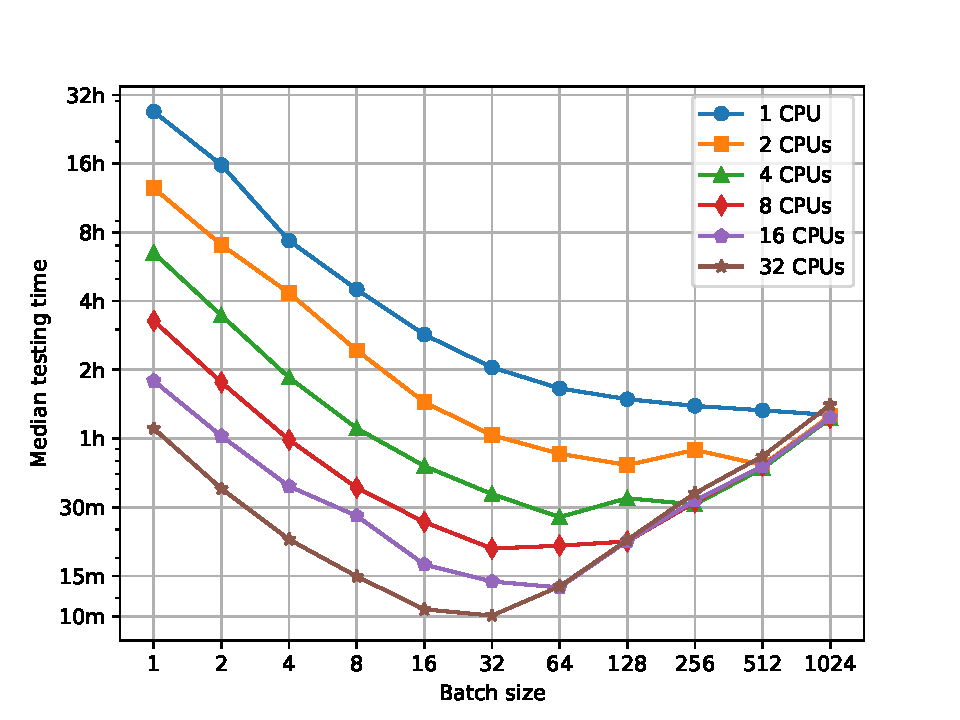
\includegraphics[trim={0.5cm 0.3cm 1.6cm 1.4cm}, clip, width=\linewidth]{images/speed-tests}
\caption{The median testing times for different numbers of \acro{CPU}s and different batch sizes}
\label{fig:results}
\end{figure}

\section{Results}
\label{sec:results}

Figure~\ref{fig:results} shows the results of our experiment. In this section, we will discuss the results and how they relate to the three research questions outlined in the previous section.

\subsection{Multiprocessing}
With batch size 1, the testing speed scales almost linearly with the number of \acro{CPU}s, as we would expect. Whereas the median testing time is 27 hours and 2~minutes with 1~\acro{CPU}, it is only 1~hour and 6 minutes with 32~\acro{CPU}s, which is about $24\times$ speed-up.\footnote{The reason why we did not achieve the theoretical $32\times$ speedup is likely due to tasks from other users that we shared our \acro{CPU}s with.}

\subsection{Batching of test files}
With 1~\acro{CPU}, the testing speed also scales almost linearly with the batch size up to a point. Whereas the median testing time is 27 hours and 2~minutes with batch size 1, it is only 4~hours and 30 minutes with batch size 8, which is about $6\times$ speed-up, and 1~hour and 20 minutes with batch size 512, which is about $21\times$ speed-up. This indicates that initialization dominates the testing time, as we expected.

To better understand the relationship between the initialization and the testing time, we can solve the following series of equations:
\begin{align*}
    10\cdot(783\cdot(X + Y)) &= \text{27h 02m} \tag{Batch size 1} \\
    10\cdot(X + 783\cdot Y) &= \text{01h 16m}  \tag{Batch size 1024}
\end{align*}
In the equations, the variable $X$ stands for the mean time that it takes to initialize a \TeX{} format and the variable $Y$ stands for the mean time that it takes to process the markdown text of a single test file.

The solution shows that whereas it takes $X\approx\text{12 seconds}$ to initialize a \TeX{} format, it takes only $Y\approx\text{0.5 seconds}$ to process the markdown text of a single test file. \emph{Without batching, 95\% of time is spent on initialization and only 5\% on actual testing. With batching, up to 97\% of time is spent on testing.}

\subsection{Batch size limiting}
% Combined speed-up of multiprocessing and batching
% The effect of batch size limiting

\section{Related work}
\label{sec:related-work}

The techniques of batching and batch splitting were perhaps first used with \TeX{} in the \acro{ARQ}Math shared evaluation tasks for the large-scale indexing of math formulae from scientific articles and Q\&A forums.

In the first \acro{ARQ}Math task, the \acro{MIRMU} team utilized the \LaTeX ML tool to convert \TeX{} formulae into the \acro{XML} format~\cite[Section~2.2]{novotny2020three}. Due to overhead issues when processing each formula separately, \acro{MIRMU} processed them in batches. However, large batches led to many formulae being lost due to errors. To mitigate this, \acro{MIRMU} used batch splitting to recover correct formulae.\footnote{See \tburl{https://github.com/MIR-MU/ARQMath-data-preprocessing}, file \texttt{scripts/latex\_tsv\_to\_cmml\_and\_pmml\_tsv.py}.} The combination of batching and batch splitting allowed \acro{MIRMU} to convert the formulae quickly and losslessly.

\section{Conclusion}
\label{sec:conclusion}

\section{Future work}
\label{sec:future-work}

\section*{Acknowledgements}

\bibliographystyle{tugboat}
\begingroup
\RaggedRight
\bibliography{main}
\endgroup

\makesignature
\end{document}
